\let\negmedspace\undefined
\let\negthickspace\undefined
\documentclass[journal]{IEEEtran}
\usepackage[a5paper, margin=10mm, onecolumn]{geometry}
%\usepackage{lmodern} % Ensure lmodern is loaded for pdflatex
\usepackage{tfrupee} % Include tfrupee package

\setlength{\headheight}{1cm} % Set the height of the header box
\setlength{\headsep}{0mm}     % Set the distance between the header box and the top of the text

\usepackage{gvv-book}
\usepackage{gvv}
\usepackage{cite}
\usepackage{amsmath,amssymb,amsfonts,amsthm}
\usepackage{algorithmic}
\usepackage{graphicx}
\usepackage{textcomp}
\usepackage{xcolor}
\usepackage{txfonts}
\usepackage{listings}
\usepackage{enumitem}
\usepackage{mathtools}
\usepackage{gensymb}
\usepackage{comment}
\usepackage[breaklinks=true]{hyperref}
\usepackage{tkz-euclide} 
\usepackage{listings}
% \usepackage{gvv}                                        
\def\inputGnumericTable{}                                 
\usepackage[latin1]{inputenc}                                
\usepackage{color}                                            
\usepackage{array}                                            
\usepackage{longtable}                                       
\usepackage{calc}                                             
\usepackage{multirow}                                         
\usepackage{hhline}                                           
\usepackage{ifthen}                                           
\usepackage{lscape}
\begin{document}

\bibliographystyle{IEEEtran}
\vspace{3cm}

\title{10.3.2.4.1}
\author{EE24BTECH11012 - Bhavanisankar G S}
% \maketitle
% \newpage
% \bigskip
{\let\newpage\relax\maketitle}

\renewcommand{\thefigure}{\theenumi}
\renewcommand{\thetable}{\theenumi}
\setlength{\intextsep}{10pt} % Space between text and floats


\numberwithin{equation}{enumi}
\numberwithin{figure}{enumi}
\renewcommand{\thetable}{\theenumi}

\textbf{QUESTION} : \\
Determine if the system of equations
\begin{align}
	x + y &= 5 \label{eq:qn} \\
	2x + 2y &= 10
\end{align}
is consistent or not. If consistent, obtain the solution graphically. \\
\textbf{SOLUTION} : \\
A linear equation is said to be \textbf{consistent} if it has atleast one solution. \\
A linear equation is said to be \textbf{inconsistent} if it has no solution. \\
Consider the given equations, 
\begin{align}
	x + y &= 5 \\
	2x + 2y &= 10
\end{align}
The equations can be written in the matrix form as, 
\begin{align}
	\myvec{1 & 1 \\ 2 & 2} \myvec{x \\ y} &= \myvec{5 \\ 10 }
\end{align}
This question can be attempted to solve using \textbf{LU decomposition} . The matrix $\vec{A}$ can be decomposed as
\begin{align}
	\vec{A} &= \vec{L} \vec{U}
\end{align}
where, 
\begin{align}
	\vec{L} &= Lower triangular \\
	\vec{U} &= Upper triangular
\end{align}
Then the system of equations can be solved as
\begin{align}
	\vec{A} \vec{x} &= \vec{B} \label{eq:solve}\\
	\vec{L} \vec{U} \vec{x} &= \vec{B} \\
	\implies \vec{L} \vec{y} &= \vec{B} \label{eq:lu1} \\
	\vec{U} \vec{x} &= \vec{y} \label{eq:lu2}
\end{align}
\textbf{Algorithm} : \\
\begin{enumerate}
	\item Let $\vec{A}$ be an $n \times n$ matrix. Initialize $\vec{L}$ to an $n \times n$ Identity matrix. Initialize $\vec{U}$ to a zero matrix.
	\begin{align}
		L &= \myvec{1 & 0 & \cdots & 0 \\
		            0 & 1 & \cdots & 0 \\
		            \vdots & \vdots & \ddots & \vdots \\
		            0 & 0 & \cdots & 1} \\
		U &= \myvec{0 & 0 & \cdots & 0 \\
			    0 & 0 & \cdots & 0 \\
                            \vdots & \vdots & \ddots & \vdots \\
                            0 & 0 & \cdots & 0}
	\end{align}
	\item For each row $i$ from $0$ to $n-1$ :
	\begin{enumerate}
		\item For each column $j$ from $i$ to $n-1$ : 
		\begin{align}
			U_{ij} &= A_{ij} - \sum_{k=0}^{i-1} L_{ik} U_{kj}
		\end{align}
		\item For each row $j$ from $i+1$ to $n-1$ :
		\begin{align}
			L_{ji} &= \frac{1}{U_{ii}} \brak{A_{ij} - \sum_{k=0}^{i-1} L_{jk} U_{ki}}
		\end{align}
	\end{enumerate}
	\item Repeat the above step for all $i = 0,1,\dots,n-1$
	\item After all the iterations
	\begin{align}
		\vec{A} &= \vec{L} \vec{U}
	\end{align}
\end{enumerate}
It can be seen that
\begin{align}
	\vec{L} &= \myvec{1 & 0 \\ 2 & 1} \\
	\vec{U} &= \myvec{1 & 1 \\ 0 & 0}
\end{align}
The matrix $\vec{U}$ can also be calculated by \textbf{Row-reduction}.
\begin{align}
	\myvec{1 & 1 \\ 2 & 2} &\xrightarrow{R_{2} \rightarrow R_{2} - 2R_{1}} \myvec{1 & 1 \\ 0 & 0} \\
	\implies \vec{U} &= \myvec{1 & 1 \\ 0 & 0}
\end{align}
The matrix $\vec{L}$ is such that the diagonal elements are 1, and is lower-triangular.
\begin{align}
	\vec{L} &= \myvec{1 & 0 \\ a & 1} \\
	\implies \myvec{1 & 0 \\ a & 1} \myvec{1 & 1 \\ 0 & 0} &= \myvec{5 \\ 10}
\end{align}
It can be seen that
\begin{align}
	a &= 2 \\
	\vec{L} &= \myvec{1 & 0 \\ 2 & 1}
\end{align}
Using \eqref{eq:lu1}, we have
\begin{align}
	\myvec{1 & 0 \\ 2 & 1} \myvec{y_{1} \\ y_{2}} &= \myvec{5 \\ 10}
\end{align}
By the method of \textbf{Forward substitution}, we have
\begin{align}
	\myvec{y_{1} \\ y_{2}} &= \myvec{5 \\ 0}
\end{align}
Similarly, 
\begin{align}
	\myvec{1 & 1 \\ 0 & 0} \myvec{x_{1} \\ x_{2}} &= \myvec{5 \\ 0} \label{eq:ans2}
\end{align}
It can be seen that
\begin{align}
	x_{1} + x_{2} &= 5 \label{eq:ans} \\
	0 &= 0
\end{align}
indicating that the given system of equations has infinite number of solutions. It can also be seen that \eqref{eq:ans} and \eqref{eq:qn} are the same. \\
Hence, the given system of equations is \textbf{consistent}. \\
Thus, any point on the line \eqref{eq:qn} is a solution to the given system of equations. \\
\textbf{Another method} : \\
The ratio of the coefficients can be seen as
\begin{align}
	\frac{1}{2} = \frac{1}{2} = \frac{5}{10}
\end{align}
Hence, the given set of equations has infinitely many solutions. \\
\textbf{QR decomposition} : \\
This question can also be solved using the \textbf{QR decomposition}. Consider
\begin{align}
	\vec{A} &= \vec{Q} \vec{R} \\
	\vec{Q} &- Orthonormal \\
	\vec{R} &- Upper triangular
\end{align}
The equation \eqref{eq:solve} can be simplified to
\begin{align}
	\vec{Q} \vec{R} \vec{x} &= \vec{B} \\
	\vec{R} \vec{x} &= \vec{Q}^{T} \vec{B}
\end{align}
Using the \textbf{Gram-Schmidt orthogonalisation}, we have
\begin{align}
	\vec{A} &= \myvec{1 & 1 \\ 2 & 2} \\
		&= \myvec{\frac{1}{\sqrt{5}} & 0 \\ \frac{2}{\sqrt{5}} & 0} \myvec{\sqrt{5} & \sqrt{5} \\ 0 & 0} \\
	\implies \myvec{\sqrt{5} & \sqrt{5} \\ 0 & 0} \myvec{x \\ y} &= \myvec{\frac{1}{\sqrt{5}} & \frac{2}{\sqrt{5}} \\ 0 & 0} \myvec{5 \\ 10}
\end{align}
which again simplifies to \eqref{eq:ans2} indicating that the given system is consistent with infinite number of solutions.

\begin{figure}[h]
\centering
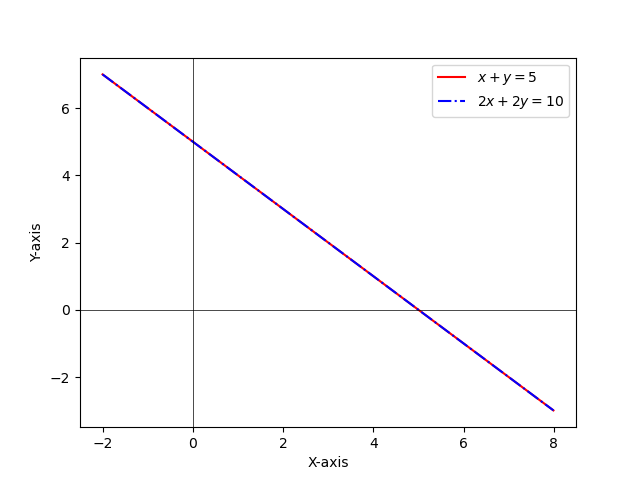
\includegraphics[width=\columnwidth]{figs/fig.png}
\caption{Plot of the given question.}
\label{fig:Plot1} 
\end{figure}
\end{document}
